\documentclass[10pt]{amsart}
\usepackage{geometry}                % See geometry.pdf to learn the layout options. There are lots.
\geometry{letterpaper}                   % ... or a4paper or a5paper or ... 
%\geometry{landscape}                % Activate for for rotated page geometry
%\usepackage[parfill]{parskip}    % Activate to begin paragraphs with an empty line rather than an indent
\usepackage{graphicx}
\usepackage{amssymb}
\usepackage{epstopdf}
\usepackage{tikz}
\usepackage{enumerate}
\DeclareGraphicsRule{.tif}{png}{.png}{`convert #1 `dirname #1`/`basename #1 .tif`.png}

\title{UVG-MM2014, Ecuaciones Diferenciales: Proyecto Extra }
\author{Carlos Eduardo L\'{o}pez Camey, carn\'{e} \#08107}\thanks{Carlos Eduardo L\'{o}pez Camey, Universidad del Valle de Guatemala, Depto. de Matem\'{a}ticas, Ecuaciones Diferenciales, Secci\'{o}n 40. http://kmels.net}

\date{Agosto del 2009}
%\date{}                                           % Activate to display a given date or no date

\begin{document}
\maketitle

% Licencia
\begin{center}

\includegraphics[scale=0.83]{img/cc/cc_by_30.pdf}\hspace*{0.95ex}
\includegraphics[scale=0.83]{img/cc/cc_sa_30.pdf}\\[1.5ex]Trabajo licenciado bajo \textit{Creative Commons Attribution-ShareAlike 3.0}.
\vspace*{1.5ex}
\end{center}

\textbf{Problema: }Un conejo est\'{a} parado en el origen. Un lobo est\'{a} en reposo, parado en la coordenada 
$(a,0)$ y en el instante $t=0$ ambos se percatan de su mutua existencia. El conejo echa a 
correr a lo largo del eje $y$ positivo con una rapidez constante $w$ mientras el lobo trata de 
alcanzarle con una velocidad que \textbf{siempre apunta} en direcci\'{o}n al conejo y con magnitud 
constante $v_0$


\begin{enumerate}[a.] 

% *********
% Inciso A
% *********
\item Haga un dibujo que represente el problema, indicando claramente las variables de 
inter\'{e}s y el sistema de referencia. Coloque al lobo en un punto intermedio de su 
trayectoria.

\vspace{1cm}
\textbf{Diagrama:}
	\begin{center}
	\begin{tikzpicture}[scale=4]
		%Recortarlo
		\clip (-0.25,-0.25) rectangle (1.65,1.65); 
		
		% Ejes
		 \draw[->] (-1.5,0) -- (1.5,0) node[right] {$x^{+}$}; 	%eje x
		 \draw[->] (0,-1.5) -- (0,1.5) node[above] {$y^+$}; 	%eje y
		
		%El Triangulo
		\filldraw[fill=green!20,draw=green!50!black] 
		(0.145,0.6) -- (0.0725,0.6) arc (180:150.55:3mm) -- cycle; 
		\draw[green!50!black]  (0.1025,0.6) node[above] {$\theta$};
		
		%Dibujar el punto desde donde parte, (a,0)
		\fill[fill=blue] (canvas cs:x=1cm,y=0cm) circle (0.5pt) node[below]{$(a,0)$};

		%Dibujar la trayectoria del lobo
		\draw [dashed,blue] (1,0) .. controls (0.4,-0) and (0.10,0.6) .. (0.15,0.6); 
		\fill[fill=blue] (canvas cs:x=0.145cm,y=0.6cm) circle (0.45pt) node[right]{$(x,y)$};
		
		%vector V_o
		\draw [->,green!50!black] (0.145,0.6) -- (0.0725,.905) node[below right]{$v_o$};
		
		%El conejo
		\draw [dashed,red] (0,0) -- (0,1); 
		\fill [fill=red](canvas cs:x=0cm,y=1.2cm) circle (0.5pt) node[right]{$(0,w)$};
		\draw [->,red] (0,1.2) -- (0,1.4) node[right]{$w$};
		
		%Leyenda
		\fill[fill=blue] (canvas cs:x=1cm,y=1.4cm) circle (0.5pt) node[right]{$Lobo$};
		\fill [fill=red] (canvas cs:x=1cm,y=1.25cm) circle (0.5pt) node[right]{$Conejo$};
	
	\end{tikzpicture} 
	\end{center}
	
%\pagebreak
% *********
% Inciso B
% *********

\item  Halle la ecuaci\'{o}n diferencial que modela la trayectoria del lobo. Escriba la 
condici\'{o}n inicial de la misma y el intervalo de validez para la variable 
independiente. �De qu\'{e} orden es la ecuaci\'{o}n? Quiz\'{a}s deba investigar un poco de 
reducci\'{o}n de orden. 
\vspace{1cm}

\textbf{Soluci\'{o}n: }Dado que la velocidad del conejo $w$ permanece constante, despu\'{e}s de un tiempo $t$, se sabe que este se encuentra en la posici\'{o}n $(0,wt)$ del plano cartesiano. El lobo se encuentra en $(x,y)$ tal y como lo ilustra el diagrama en el inciso (a).

Procedamos a calcular entonces $\frac{dy}{dx}$ para el modelo. Sabemos que

\[ \frac{dy}{dx} = \frac{\frac{dy}{dt}}{\frac{dx}{dt}} \]

En donde, calculando $\frac{dy}{dt}$ y $\frac{dx}{dt}$, las velocidades $v_o$ del lobo en el eje $y$ y en el eje $x$ respectivamente, tenemos que

\[\frac{dy}{dt} = v_o\cdot \text{sin}\theta = v_o \cdot \frac{wt - y}{\sqrt{x^2 + (wt-y)^2}}\]

y 

\[\frac{dx}{dt} = v_o\cdot \text{cos}\theta = v_o \cdot \frac{-x}{\sqrt{x^2 + (wt-y)^2}}\]

Por lo tanto, re-escribiendo

\begin{equation}
\frac{dy}{dx} = \frac{v_o\cdot \frac{wt - y}{\sqrt{x^2 + (wt-y)^2}}}{v_o \cdot \frac{-x}{\sqrt{x^2 + (wt-y)^2}}} = -\frac{wt-y}{x} \implies -x\frac{dy}{dx} = wt - y \:\:\: \text{con}  \: x \neq 0
\end{equation}

Derivando (1) respecto a $x$, tenemos que

\[ - \frac{dy}{dx} + x\frac{d^2y}{dx^2} = w\frac{dt}{dx} - \frac{dy}{dx} \implies x\frac{d^2y}{dx^2} = w\frac{dt}{dx}\]

En donde, $t$ no depende de $x$ pero $x$ si depende de $t$, y conocemos $\frac{dx}{dt}$, entonces, re-escribiendo y por el teorema de la funci\'{o}n inversa:

\begin{equation} \frac{1}{x\frac{d^2y}{dx^2}} = \frac{1}{w}\frac{dx}{dt} \implies \frac{dx}{dt} = \frac{w}{x\frac{d^2y}{dx^2}} \:\:\: \text{con}  \: w \neq 0
\end{equation}

Como dijimos antes, conocemos $\frac{dx}{dt}$, entonces 

\[ \frac{-x v_o}{\sqrt{x^2+(wt-y)^2}} = \frac{w}{x\frac{d^2y}{dx^2}}  \]

\[ \frac{-x v_o}{\sqrt{x^2+(wt-y)^2}} = \frac{w}{x\frac{d^2y}{dx^2}}  \]

Re-escribiendo de nuevo

\[ x \frac{d^2y}{dx} = \frac{w}{-xv_o} \cdot \sqrt{x^2+(wt-y)^2} \:\:\: \text{con} \: v_o \neq 0 \]

\[ x \frac{d^2y}{dx} = \frac{w}{v_o} \cdot \sqrt{\frac{1}{x^2}\cdot[x^2+(wt-y)^2]}\]

\[ x \frac{d^2y}{dx} = \frac{w}{v_o} \cdot \sqrt{1+\frac{(wt-y)^2}{x^2}}\]

\[ x \frac{d^2y}{dx} = \frac{w}{v_o} \cdot \sqrt{1+ \displaystyle{(\frac{dy}{dx} )^2}}\]

Que es el modelo que quer\'{i}amos encontrar.   \\ 

Este modelo est\'{a} sujeto a que, tanto la velocidad del conejo como la del lobo, y la posici\'{o}n $x$ del lobo sean distintas de 0. Es notable ya que, en este caso, no habr\'{i}a persecuci\'{o}n o esta se volver\'{i}a un simple problema de f\'{i}sica (en el caso que x=0)
\\ \\
El intervalo de validez para la variable independiente $x$ es, (- $\infty$,0) \'{o} bien (0, $\infty$).
\vspace{1cm}

% *********
% Inciso C
% *********
\item Halle la soluci\'{o}n de la ecuaci\'{o}n diferencial. Utilice  la constante $k = \frac{w}{v_o}$

\vspace{1cm}

\textbf{Soluci\'{o}n: }Sabiendo que el modelo es una ecuaci\'{o}n de segundo orden, usaremos la t\'{e}cnica de reducci\'{o}n de orden, la cual consiste en, como su nombre lo dice, reducir el orden de una ecuaci\'{o}n diferencial.
\\
Haciendo $p = \frac{dy}{dx}$, implica que $\frac{dp}{dx} = \frac{d^2y}{dx^2}$. Entonces

\[x \frac{dp}{dx} = k \sqrt{1+p^2} \]

Que, cambiando la notaci\'{o}n y resolviendo por separaci\'{o}n de variables, tenemos

\[ \int \frac{1}{\sqrt{1+p^2}} \: dp = k \int \frac{1}{x} \: dx\]

\[ \sinh ^{-1}(p) = k \: \ln{(x)} + c \]

Por propiedades de logaritmos, sabemos que $k \: \ln{(x)} = \ln{(x^k)}$ y sabiendo que c es una constante, hacemos $c = \ln{(c_1)}$. Entonces

\begin{equation}
 p = \sinh{\displaystyle [ \ln{(x^k)} + \ln{(c_1)} ] } = \sinh{\displaystyle [ \ln{(\frac{x^k}{c_1})}] = \sinh{[\displaystyle{\ln{(c_2 \: x^k)}}]} } 
 \end{equation}

Haciendo uso de la definici\'{o}n de $\sinh$, re-escribimos (3)

\[ \frac{1}{2} \displaystyle{(  e^{\ln{(c_2 \: x^k)}} - e^{-\ln{(c_2 \: x^k)}}   ) } = \frac{1}{2} \displaystyle{(c_2\:x^k - \frac{1}{c_2\:x^k})} =  \frac{dy}{dx} \]

Sabemos que en $t=0$, $\frac{dy}{dx} = 0$ y $x$, la posici\'{o}n del lobo, es $a$. Entonces para \'{e}ste caso podemos escribir

\[
\frac{1}{c_2 x^k} = c_2x^k \implies (c_2)^2 = \frac{1}{a^{2k}} \implies c_2 = \frac{1}{a^k}
\]

Entonces, tenemos nuestra ecuaci\'{o}n diferencial reducida

\begin{equation}
\frac{dy}{dx} = \frac{1}{2}[ \frac{x^k}{a^k} - \displaystyle{\frac{a^k}{x^k}}]
\end{equation}

Resolviendo por separaci\'{o}n de variables

\[ \int dy = \frac{1}{2} \int [ \frac{x^k}{a^k}  - \frac{a^k}{x^k} ] dx \] 

\textbf{Caso 1:} Si $k\neq1$, entonces
\[ y = \frac{1}{2} [\frac{x^{k+1}}{a^k (k+1)} - \frac{a^k x^{1-k}}{1-k}] + d\]

De nuevo, sabemos que en $t=0$, $x=a$ y $y=0$. Por lo tanto,

\[ 0 = \frac{1}{2} [\frac{a^{k+1}}{a^k(k+1)}-\frac{a^ka^{1-k}}{(1-k)}] + d \]

Re-escribimos por propiedades de exponentes
\[ 0 = \frac{1}{2} [\frac{a^ka}{a^k(k+1)}-\frac{a^ka^{-k}a}{(1-k)}] + d\]

\[ 0 = \frac{1}{2} [\frac{a}{k+1}-\frac{a}{-k+1}] + d\]

Despejando para $d$
\[ - d = \frac{a\cdot -2k}{2(1-k^2)} \implies d = \frac{a\cdot k}{(1-k^2)} \] 

Escribiendo la soluci\'{o}n completa para el caso 1

\begin{equation}
y = \frac{1}{2} [\frac{x^{k+1}}{a^k (k+1)} - \frac{a^k x^{-k+1}}{1-k}] + \frac{a\cdot k}{1-k^2}
\end{equation}

en donde $k = \frac{w}{v_o} \neq 1$\\

\textbf{Caso 2:} Si $k = 1$, planteando la integral
\[ \int dy = \frac{1}{2}\int [\frac{x}{a} - \frac{a}{x}]dx\]

Resolviendo, tenemos 
\[ y = \frac{1}{2} [\frac{x^2}{2a} - a\cdot \ln x ] + h\]

De nuevo, haciendo uso de que en $t=0$, $x=a$ y $y=0$
\[ 0 = \frac{1}{2} [\frac{a^2}{2a} - a\cdot \ln a ] + h \implies h =  \frac{1}{2} [ a\ln a - \frac{a}{2} ] \]

Escribiendo la soluci\'{o}n completa para el caso 2

\[
y = \frac{1}{2} [\frac{x^2}{2a} - a\cdot \ln x ] + \frac{1}{2} [ a\ln a - \frac{a}{2}]
\]

Finalmente, simplificando un poco, tenemos
\begin{equation}
y = \frac{1}{2} [\frac{x^2}{2a} - a\cdot \ln x  + a \cdot \ln a  - \frac{a}{2} ]
\end{equation}

en donde $k = \frac{w}{v_o} =  1$\\
% *********
% Inciso D
% *********
\item Analice qu\'{e} sucede para el caso cuando $v_o < w$

\vspace{1cm}
\textbf{An\'{a}lisis: }Si $v_o < w$ entonces, $k > 1$. Tenemos para (5)
\[ y = \frac{1}{2} [\frac{x^{k+1}}{a^k (k+1)} - \frac{a^k x^{1-k}}{1-k}] + \frac{a\cdot k}{1-k^2}\]

que el primer t\'{e}rmino, $\frac{x^{k+1}}{a^k(k+1}$ es menor que el segundo, $\frac{a^k x^{1-k}}{1-k}$, eso se debe a que el $x^{1-k}$ que aparece en el segundo, en realidad es $\frac{1}{x^{k-1}}$ y con $k>1$, este es mayor. El tercer y \'{u}ltimo t\'{e}rmino es una constante.\\

El \'{u}ltimo enunciado nos dice que $x$ en (6) se indefine en $0$. Si analizamos $ \displaystyle \lim_{x \to 0^+} y$, tendremos que \'{e}ste tiende a $\infty$. Por lo tanto, el lobo no alcanzar\'{i}a al conejo jam\'{a}s en esta situaci\'{o}n

\vspace{1cm}
% *********
% Inciso E
% *********
\item Analice qu\'{e} sucede para el caso cuando $v_o = w$

\vspace{1cm}
\textbf{An\'{a}lisis: }Si $v_o = w$ entonces, $k = 1$. Tomemos (6):

\[ y = \frac{1}{2} [\frac{x^2}{2a} - a\cdot \ln x  + a \cdot \ln a  - \frac{a}{2} ]\]

Claramente, la funci\'{o}n se indefine, como en el inciso (d), significando que el lobo nunca alcanzar\'{a} al conejo si los dos tienen la misma velocidad en la persecuci\'{o}n.

\vspace{1cm}
% *********
% Inciso F
% *********
\item Analice qu\'{e} sucede para el caso cuando $v_o > w$

\vspace{1cm}
\textbf{An\'{a}lisis: }Si $v_o < w$ entonces, $k < 1$. Tenemos para (5)
\[ y = \frac{1}{2} [\frac{x^{k+1}}{a^k (k+1)} - \frac{a^k x^{1-k}}{1-k}] + \frac{a\cdot k}{1-k^2}\]

N\'{o}tese que al contrario de los dos incisos anteriores, esta soluci\'{o}n no se indefine para ning\'{u}n $x$, por lo tanto, se podr\'{i}a despejar para esta y descubrir en que punto las trayectorias del conejo y del lobo se intersectan, es decir, cuando el lobo alcanza al conejo.\\

Si evaluamos para $x=0$ tenemos

\begin{equation}
y = \frac{1}{2} (\frac{0}{a^k(k+1} - \frac{0}{-k+1}) + \frac{a\cdot k}{1-k^2} = \frac{a\cdot k}{1-k^2}
\end{equation}

el punto en donde el lobo lo alcanza.
\vspace{1cm}
% *********
% Inciso G
% *********
\item Grafique la trayectoria del lobo para los casos planteados en los incisos (d), (e) y 
(f). Para este efecto deber\'{a} asignar valores num\'{e}ricos apropiados para todas las 
constantes.\\

\textbf{Grafica inciso (d): } Tomando en cuenta que un lobo puede correr hasta 35mph \cite{Wolfspeed} y el conejo, unos 45 mph\cite{Conejospeed}, consideremos el caso cuando el conejo tiene una velocidad $w$ de 40mph y el lobo de 20mph.

Suponiendo que el lobo parte 25 millas hacia el este del conejo y calculando $k$, tenemos $k=2$, por lo que la trayectoria del lobo estar\'{i}a dada por

\begin{equation}
y = \frac{1}{2} [\frac{x^{2+1}}{25^2 (2+1)} - \frac{25^2 x^{-2+1}}{1-2}] + \frac{25\cdot 2}{1-2^2} = \frac{1}{2} [ \frac{x^3}{25^2\cdot 3} + \frac{25^2}{x}] - \frac{50}{3}
\end{equation}

Graficando (8) tenemos:

\begin{center} 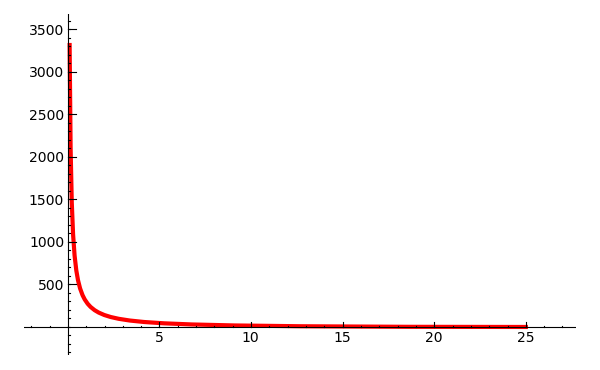
\includegraphics[scale=0.5]{img/figd1.png}\end{center}

\textbf{Grafica inciso (e): } En el caso que los dos tengan la misma velocidad, $k=1$. Suponiendo que el lobo parte 25 millas al este del coenjo, entonces evaluando para (6)

\[ y = \frac{1}{2} [\frac{25^2}{2\cdot 25} - 25\cdot \ln 25  + 25 \cdot \ln 25  - \frac{25}{2} ]\]

\begin{center} 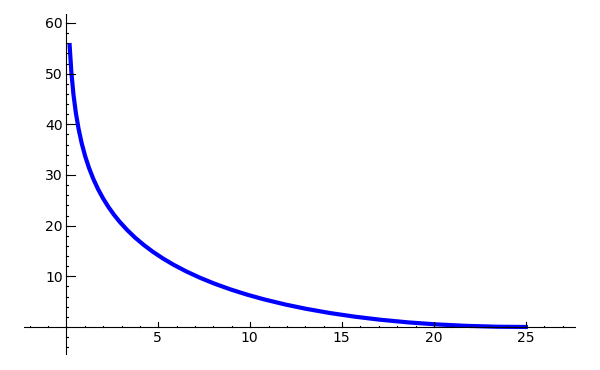
\includegraphics[scale=0.5]{img/figf1.png}\end{center}

\textbf{Grafica inciso (f): } Tomemos $w = 15$ mph y $v_o = 30$mph, eso implicar\'{i}a $k=0.5$. Con el lobo partiendo 25 millas al oeste del conejo tenemos:

\begin{equation}
y = \frac{1}{2} [\frac{x^{0.5+1}}{25^{0.5} (0.5+1)} - \frac{25^{0.5} x^{-0.5+1}}{1-0.5}] + \frac{25\cdot 0.5}{1-0.5^2} = \frac{1}{2}[ 2\frac{x\sqrt{x}}{5\cdot 3} + \frac{2\cdot 5 \cdot \sqrt{x}}{1}] + \frac{12.5}{0.75} 
\end{equation}

Graficando (9)
\begin{center} 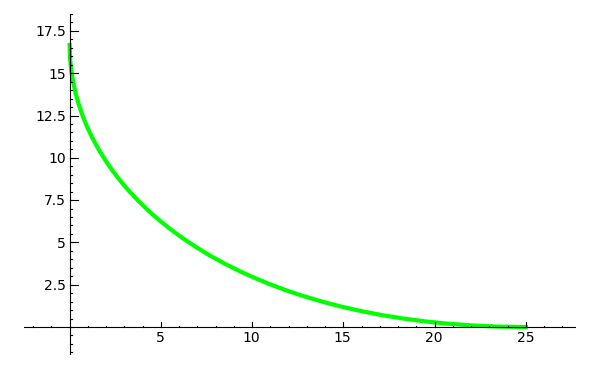
\includegraphics[scale=0.5]{img/fige1.png}\end{center}

%\begin{equation}
%y = \frac{1}{2} [\frac{x^{k+1}}{a^k (k+1)} - \frac{a^k x^{-k+1}}{1-k}] + \frac{a\cdot k}{1-k^2}
%\end{equation}
% http://www.wolfcountry.net/information/WolfObserved.html#speed
% http://www.ehow.com/about_4605256_how-fast-does-rabbit-run.html


\vspace{1cm}
% *********
% Inciso H
% *********
\item Asignando valores apropiados para las constantes, y para el caso $v_o > w$ halle el 
momento en el que el lobo alcanza al conejo.

\vspace{1cm}
Suponiendo $vo = 30$ mph y $w = 15$ mph, tenemos $k=0.5$. Si la distancia $a$ que separa  al lobo del conejo en sus partidas es 1 milla, entonces evaluando para (7) tenemos

\[ y = \frac{1 \cdot 2}{1-0.5^2} = \frac{2}{0.75}  \approx 2.66 \: \text{millas} \]

Sabiendo que la velocidad $w$ del conejo es constante en toda la persecuci\'{o}n, calculando $t$

\[ t = \frac{y}{w} = \frac{2.66 \: \text{millas}}{\frac{15 \: \text{millas}}{\text{hora}}} \approx 0.18 \text{horas} \approx 10.8 \: \text{minutos} \]

Que es lo que quer\'{i}amos encontrar para las condiciones dadas.
\end{enumerate}

%\section{}
%\subsection{}

\begin{thebibliography}{2}
  \bibitem{Wolfspeed} Wolf Facts, WolfCountry.Net, http://www.wolfcountry.net/information/WolfObserved.html\#speed
  \bibitem{Conejospeed} How Fast does a Rabbit Run?, eHow.com, http://www.ehow.com/about\_4605256\_how-fast-does-rabbit-run.html
 \end{thebibliography}


\end{document}  